\section{Expectation Maximization Algorithms}
\label{sec:expect-max-algos}
The previous section has established the equivalence between the K-Means problem and the problem of the optimal tree, formulated in \eqref{eq:symbolic-optimization-with-minflow2}.
In this section, the K-means algorithm is further explained in section \ref{sec:k-means-standard}.
Building on this analysis, an algorithm to generate optimal trees based on the K-Means algorithm is devised.
Promising results are reported in section \ref{sec:kmeans-results} for this new algorithm, both for speed as well as quality of the approximation. 

In section \ref{sec:k-means-as-EM}, the relationship between the K-Means algorithm and Expectation Maximization algorithms is explained.
Building on this relationship, the discretization of the infinite dimensional Kantorovich distance introduced in section \ref{sec:math-foundations} is revisited.
It is found that the discretization in fact exhibits a hidden prior/bias on the distribution.
\subsection{The K-Means Algorithm}
\label{sec:k-means-standard}
In this section, the K-Means algorithm briefly introduced in \ref{sec:kantorovich-and-clusters} will be discussed in detail.

The K-Means algorithm is usually thought of in the framework of unsupervised data mining.
Given a set of unlabeled data $X$, the goal is to find labels $Y$ for every $x\in X$, such that the data points with common labels meet some form of homogeneity criterion.
The space $U\supset X$ is generally endowed with some measure of dissimilarity $c: X\times U\rightarrow \mathbb{R}_+$.
The homogeneity criterion is expressed in terms of the dissimilarity between the elements of a cluster (that is all $x\in X$ that share the same label $y\in Y$) and the ``centroid'' $\mu\in U$ of the cluster.
The two most common choices for $U$ are $U=\mathbb{R}^n$ and  $U=X$.
These choices correspond to the K-Means and the K-Medoids algorithms from the previous section.
The general procedure is independent of this choice.

The algorithm demands the number of different labels $K=|Y|$ as an input parameter.
We introduce binary assignment variables $z_{ij}$ which are one, if label $y_j$ is attached to data point $x_i$, and zero otherwise. 
Obviously, 
\[\sum_{j\in Y}z_{ij} = 1\]
has to hold.
Using these labels, we can define the objective function (sometimes known as the ``distortion function'' for the K-Means problem as
\begin{equation}
  \label{eq:5}
  J(z, \mu) = \sum_{i}\sum_{j}z_{ij}c(x_i, \mu_j).
\end{equation}
The K-Means problem can be expressed as
\begin{equation}
  \label{eq:3}
  \min\limits_{z, \mu}J(z, \mu).
\end{equation}
This mixed integer optimization problem is in general intractable, due to the often large number of data points.
The problem, though hard to solve to global optimality, can be solved quite efficiently using coordinate descent.
Note that the optimization of $J$ with respect to each single variable is very easy.
The solution for the assignment variables is
\begin{equation}
  \label{eq:4}
  z_{ij} = \left\{\begin{array}{ll}1&\text{if }j=\underset{i}{\argmin}\; c(x_i,\mu_j)\\0&\text{otherwise} \end{array}\right. .
\end{equation}
For the centroids, this depends on the choice of $U$ and $c$.
For the case of $U=\mathbb{R}^n$, $c(x,\mu) = \Vert x-\mu\Vert^2$ it becomes the solution to a quadratic equation
\begin{equation}
  \label{eq:6}
  \mu_j = \left(\sum_{i}z_{ij}x_{ij}\right)\left / \left(\sum_{ij}z\right)\right. .
\end{equation}
For $U=X$ and an arbitrary dissimilarity measure $c$, there is no general analytic solution, so all distance pairs $c(x_i, x_j)$ have to be evaluated:
\begin{equation}
  \label{eq:7}
  \mu_j = \underset{\hat{\mu}\in X}{\argmin}\; \sum_{i}\sum_{j}z_{ij}c(x_i,\hat{\mu})
\end{equation}
This is generally not considered to be a significant drawback, since many strategies have been found to limit the number of evaluations in actual implementations.

The algorithm is composed of alternating optimizations of J with respect to $z$ and $\mu$.
At every iteration, the objective function is guaranteed to decrease.
There is no guarantee that the value that the algorithm converges to is a global optimum.
However, If some care is taken at the initialization of the variables, in practice the algorithm generally yields nearly optimal values \cite{Arthur2006}.
The procedure is outlined below in algorithm \ref{alg:k-means}.
\begin{algorithm}
  \label{alg:k-means}
  \caption{K-Means/K-Medoids Expectation Maximization}
  \KwIn{Metric $c$, data points $X = \{x_1,\ldots , x_N\}$.}
  \KwOut{Cluster means $M=\{m_1,\ldots , m_K\}$, assignments $z_{ij}$ mapping $X\rightarrow M$.}
  \lIf{K-Means}{$U = \mathbb{R}^n$\;}
  \lIf{K-Medoids}{$U = X$\;}
  
  (Randomly) initialize $m_i$\;
  \While{$z_{ij}$ change}{
    $z_{ij}\leftarrow \left\{\begin{array}{ll} 1 & \text{if }j = \underset{k}{\argmin}\; c(x_i, \mu_k)\\0&\text{otherwise}\end{array}\right.$\tcc*{Expectation step}
    $\mu_j\leftarrow \underset{\hat{\mu}\in U}{\argmin}\; \sum_{i}\sum_{j}z_{ij}c(x_i,\hat{\mu})$\tcc*{Maximization step}
  }
\end{algorithm}
\subsection{The K-Means Algorithm for Trees}
\label{sec:k-means-algorithm-trees}
In section \ref{sec:kantorovich-and-clusters}, we showed that constructing the optimal discrete random variable $\nu$ that best approximates a given discrete uniformly distributed random variable $\xi$ is equivalent to solving the K-Means problem.
This approach does not directly apply to the tree structured stochastic processes.
In this section, we will translate the coordinate descent algorithm described in the previous section to the specific case of constructing tree-shaped discrete stochastic processes.
%
\subsubsection{Tree Representation}
Different representations of the properties of the tree are possible. A tree is completely defined by the following items:
\begin{itemize}
\item A set of node values of the tree $y_n,\, n\in N$. The node values $y_n$ represent the degrees of freedom of the tree.
\item A set of stages $t\in T$.
\item A set of scenarios of the tree $\nu_j^t,\, j\in J,\, t\in T$.
  A tree scenario is a vector of node values when traversing the tree along the branches from the root to a leaf.
\item A mapping $n: J\times T\rightarrow N$ that maps  a pair of scenario and time stage to a node.
  The values $\nu_j^t$ are defined by
  \begin{equation}
    \label{eq:9}
    \nu_j^t = y_{n(j,t)}\;\forall\, j\in J,\, t\in T
  \end{equation}
\end{itemize}
The translation of theorem \ref{thm:kmeans-kantorovich} is based on the interpretation of the scenario set $J$ of the tree as a discrete random variable.
\subsubsection{The Algorithm}
Consider now a set of scenarios $\xi_i,\, i\in I$ sampled from the original stochastic process.
These scenarios will be regarded as the uniformly distributed discrete events of the random variable that is supposed to be approximated. 
The dissimilarity measure $c$ used in the objective function (``distortion function'') depends on the feasibility set (see section \ref{sec:tree-feas-sets}) the tree has to satisfy.
For the discrete-event set, which demands that $\{\nu_j^t\}\subset\{\xi_i^t\}$, there are basically no restrictions.
For the continuous-event set, its optimal value has to be easily computable, so using the squared Euclidean norm is advisable.
In analogy to \eqref{eq:5}, assignment variables $z$ are used to link the Monte-Carlo scenarios to the tree scenarios.
The objective function is
\begin{equation}
  \label{eq:8}
  J(z, y) = \sum_{i\in I}\sum_{j\in J}z_{ij}c(\xi_i, \nu_j).
\end{equation}
The difficulty of the current problem is, that in contrast to the random variable events, the events $\nu_j$ of the tree are not independent.
Instead, they are defined by \eqref{eq:9} as functions of the node values.
The problem will again be solved using coordinate descent.
The optimization with respect to the assignment variables z is again simple. For fixed $y$, similar to \eqref{eq:4} we have
\begin{equation}
  \label{eq:10}
  z_{ij} = \left\{\begin{array}{ll}1&\text{if }j=\underset{i}{\argmin}\; c(\xi_i,\nu_j(y))\\0&\text{otherwise} \end{array}\right. .  
\end{equation}
The optimization with respect to the node values $y$ seems at first glance more difficult, but will prove to be just as easy as with random variables. We will first consider the problem for continuous-event trees. As discussed above we choose $c(\xi, \nu) = \Vert \xi-\nu\Vert^2$ as the dissimilarity function. The solution to
\begin{equation}
  \label{eq:11}
  \min\limits_y J(z,y) = \min\limits_y \sum_{i\in I}\sum_{j\in J}z_{ij}\Vert \xi_i - \nu_j\Vert^2
\end{equation}
As we are dealing with an unconstrained, convex, differentiable optimization problem, the minimum is attained at the zero of the derivative. For node $k$ this means
\begin{equation}
  \label{eq:12}
  \frac{\partial J(z,y)}{\partial y_k} = \sum_{i\in I}\sum_{j\in J}z_{ij}\frac{\partial c(\xi_i, \nu_j^t)}{\partial y_k}\overset{!}{=} 0.
\end{equation}
The derivative can be expanded to
\begin{equation}
  \label{eq:13}
  \frac{\partial c(\xi_i, \nu_j^t)}{\partial y} = \frac{\partial c(\xi_i, \nu_j^t)}{\partial \nu_j^t}\frac{\partial \nu_j^t}{\partial y_k}.
\end{equation}
From \eqref{eq:9} we have
\begin{equation}
  \label{eq:14}
  \frac{\partial \nu_j^t}{\partial y_k} = 
  \left\{
    \begin{array}{ll}
      1&\text{if } k = n(j,t)\\0&\text{otherwise}
    \end{array}
  \right. .
\end{equation}
Using the definition, we finally have 
\begin{align}
  \label{eq:15}
  y_k = \left(\sum_{i\in I}\sum_{(j,t)\in n^{(-1)}(k)}z_{ij}\xi_i^t \right) \left / \left(\sum_{i\in I}\sum_{(j,t)\in n^{(-1)}(k)}z_{ij}\right)\right. ,
\end{align}
with the set $n^{(-1)}(k)$ of all pairs of scenarios $j$ and time steps $t$ that belong to this node.
In other words, the optimal value of a node is the average value of all scenarios that are associated with this node through the variables $z_{ij}$ at the time step of the node.
Note that this is almost the same as the optimal solution to the regular K-Means algorithm \eqref{eq:6}.
This completes the steps of the algorithm for continuous-event trees.

For discrete-event trees, as long as the dissimilarity function $c$ is chosen such that it can be expressed as 
\begin{equation}
  \label{eq:16}
  c(\xi_i, \nu_j) = \sum_{t\in T}c_t(\xi_i^t,\nu_j^t),
\end{equation}
the variables $y$ can similarly be computed stage-wise as the optimal nodes of 
\begin{equation}
  \label{eq:17}
  y_k = \underset{\{l\in I|\exists (j,t)\in n^{(-1)}(k):z_{lj}=1\} }{\argmin}\; \sum_{i\in I}\sum_{(j,t)\in n^{(-1)}(k)}z_{ij}c(\xi_i^t, \xi_l^t).
\end{equation}
This is the optimal value of a scenario selected among all the scenarios that were associated with this specific node.
\subsubsection{Results}
\label{sec:kmeans-results}
In this section we will present preliminary computational results. The algorithm was implemented in {\sc matlab}.

\begin{figure}
  \centering
  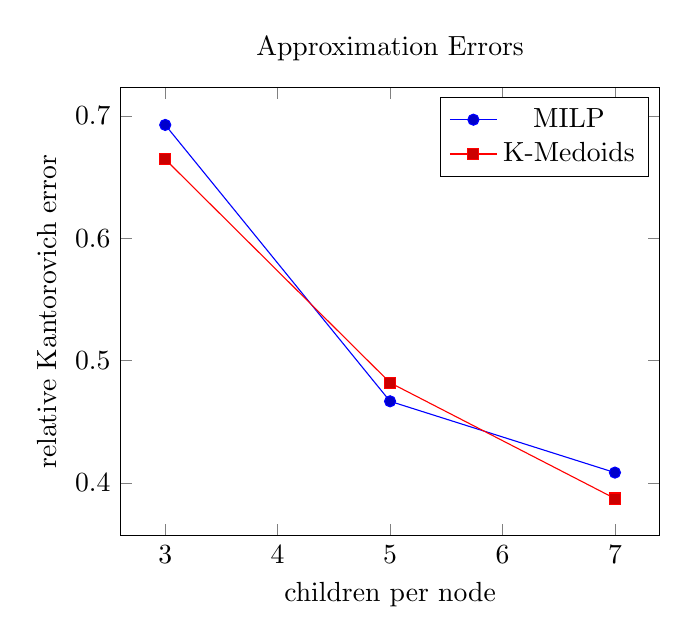
\begin{tikzpicture}
    \begin{axis}% Errors over number of children
      [
      title=Approximation Errors,
      legend entries={MILP,K-Medoids},
      xlabel=children per node,
      ylabel=relative Kantorovich error
      ]
      \addplot coordinates { % testscen=1000
        (3, 0.6927)
        (5, 0.4667)
        (7, 0.4084)
      };
      \addplot coordinates { % testscen=3000
        (3, 0.6646)
        (5, 0.4819)
        (7, 0.3872)
      };
    \end{axis}
  \end{tikzpicture}
    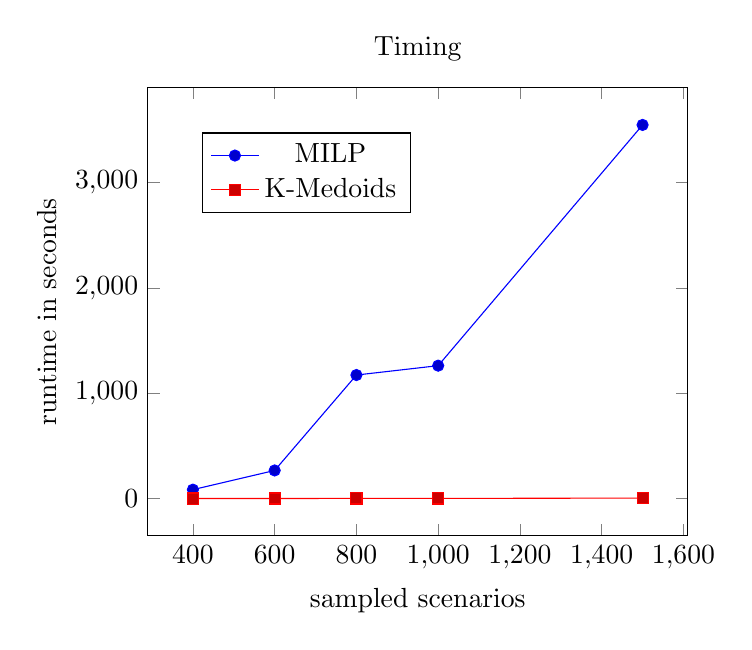
\begin{tikzpicture}
    \begin{axis}% Timing, nchildren=3,nstages=3
      [
      title=Timing,
      legend entries={MILP,K-Medoids},
      xlabel=sampled scenarios,
      ylabel=runtime in seconds,
      legend style={at={(0.1,0.9)},anchor=north west}
      ]
      %\addplot coordinates { % testscen=3000, time in seconds
      %  (3, 32.2653)
      %  (5, 39.2829)
      %  (7, 71.1328)
      %};
      \addplot coordinates{ % MILP
        (400, 85.1)
        (600, 267.4)
        (800, 1172.9)
        (1000, 1261.9)
        (1500, 3546.5)
      };
      \addplot coordinates { % K-medoids
        (400, 0.9120)
        (600, 1.3498)
        (800, 1.9716)
        (1000,1.7055)
        (1500,5.3441)
      };
    \end{axis}
  \end{tikzpicture}
  \caption{Comparison of the stage-wise MILP and K-Medoids algorithm. The figures show that the }
  \label{fig:compare-milp-kmedoids}
\end{figure}
%%% Local Variables: 
%%% mode: latex
%%% TeX-master: "da"
%%% End: 

\subsection{K-Means as an Expectation Maximization Algorithm}
\label{sec:k-means-as-EM}
In this section, we will introduce the Expectation Maximization (EM) algorithm due to \cite{Dempster1977}.

\subsubsection{A Continuous Approach for the Kantorovich Distance}
\label{sec:cont-appr-kant}
Consider the K-Means algorithm of the previous section.
There, each data-point was assigned uniquely to one of the K data clusters.
These hard assignments stem from the fact that the algorithm operates on the discretized sample $\{\xi,\, i\in I\}$ of the original stochastic process.
In a probabilistic context such as the scenario tree generation, these hard assignments are difficult to justify.
Instead of a discretization in terms of a discrete probability distribution (samples), we will analyze the approximation in a parametric function space.
The most natural parametric function space that has favourable analytic properties are sums of Gaussian distributions.
Given a set of samples $\{\xi_n,\, n\in I\}$ we assume that these originally formed the probability distribution
\begin{equation}
  \label{eq:31}
  p(x) = \sum_{n=1}^N\frac{1}{N}\mathcal{N}(x|\xi_n,\sigma_n)
\end{equation}
with the Normal distribution $\mathcal{N}$.
Since we assume that the data form a weighted sum of Normal distributions, we will replace the cluster centroids of the X-Means model with Normal distributions as well. The resulting distribution is
\begin{equation}
  \label{eq:32}
  q(x) = \sum_{k=1}^K\pi_k\mathcal{N}(x|\mu_k, \sigma_k)
\end{equation}
The parameters $\mu_k$, $\sigma_k$ and $\pi_k$ are the variables of the model.
The Kantorovich distance of the distributions $p$ and $q$ is
\begin{equation}
  \label{eq:33}
  D_K(p,q) = \min\limits_{\eta}\int\limits_{-\infty}^{\infty}\int\limits_{-\infty}^{\infty}(x-y)^2\eta(x,y)dxdy,\; \int\limits_{-\infty}^{\infty}\eta(x,y)dx = q(y),\;\int\limits_{-\infty}^{\infty}\eta(x,y)dy = p(x)
\end{equation}
For the given Gaussian functions, for one cluster $k$ (with fixed parameters) and one sample $n$, the Kantorovich metric can be explicitly computed as
\begin{equation}
  \label{eq:34}
  D(p_n,q_k) = \int\limits_{-\infty}^{\infty}\left(x-\left(\sqrt{\frac{\sigma_n}{\sigma_k}}(x-\mu_k)+\mu_n\right)\right)^2\mathcal{N}(x|\mu_k,\sigma_k)dx.
\end{equation}
See figure \ref{fig:kantoro_gauss_explain} for an illustration how the above formula relates to the distributions.
\newcommand{\fdst}[7]{%mu, sigma, outer bounds, start of marker, scale, y
  % shade the critical region tail
  \draw[fill,orange]  (#4+#1,#6) node[below]{#7}-- plot[domain=(#4+#1):(#4+#1+0.2*#2),samples=50]
  function {#6+#5*1/sqrt(2*3.1416*#2)*exp(-(x-#1)*(x-#1)/2/#2)}
  -- (#4+#1+0.2*#2,#6) -- cycle;

  % draw the F distribution curve
    \draw[color=blue!50!black,thick]
        plot[smooth,domain=(-#3+#1):(#3+#1),samples=100]
        function {#6+#5*1/sqrt(2*3.1416*#2)*exp(-(x-#1)*(x-#1)/2/#2)};


    % draw the F axis
        %\draw[->] (-#3,0) -- (#3,0) node[right] {$F$};
    % label the critical region boundary
        %    \draw (0,0) -- (#1,-0.02) node[below] {$#1$};
    % label 0
%    \draw (0,0) -- (0,-0.02) node[below] {$0$};

    % draw the y axis
 %   \draw[very thin,->] (0,0) -- (0,#5/2);
}

\begin{figure}
  \centering
  \begin{tikzpicture}
    \draw[fill,orange]  (1+0,5) node[below]{$x$}-- plot[domain=(1+0):(1+0+0.2*2),samples=50]
  function {5+4*1/sqrt(2*3.1416*2)*exp(-(x-0)*(x-0)/2/2)}node(topnische)[above, left]{}
  -- (1+0+0.2*2,5)  -- cycle;

  % draw the F distribution curve
  \draw[color=blue!50!black,thick]
  plot[smooth,domain=(-5+0):(5+0),samples=100]
  function {5+4*1/sqrt(2*3.1416*2)*exp(-(x-0)*(x-0)/2/2)} node[above] {$\mathbb{P}(x)$};



%    \fdst{0}{2}{5}{1}{3}{5}{$x$};
    % draw upper x- axis
  \draw[->] (-5,5) -- (8.2,5);

    \draw[fill,orange]  (0.707+5,0) node[below]{$ y=\sqrt{\frac{\sigma_n}{\sigma_k}}(x-\mu_k)+\xi_n$} --  plot[domain=(0.707+5):(0.707+5+0.2*0.5),samples=50]
  function {0+5*1/sqrt(2*3.1416*0.5)*exp(-(x-5)*(x-5)/2/0.5)} node(bottomnische)[below]{}
  -- (0.707+5+0.2*0.5,0)  -- cycle;

  % draw the F distribution curve
    \draw[color=blue!50!black,thick]
        plot[smooth,domain=(-3+5):(3+5),samples=100]
        function {0+5*1/sqrt(2*3.1416*0.5)*exp(-(x-5)*(x-5)/2/0.5)} node[above]{$\mathbb{Q}(y)$};

        % \fdst{5}{0.5}{3}{0.707}{5}{0}{{$ y=\sqrt{\frac{\sigma_2}{\sigma_1}}(x-\mu_1)+\mu_2$}};
        \draw[->] (-5,0) -- (8.2,0);

        \path[->,thick, color=blue!50] (topnische) edge[bend right] node[right]{$\eta(x,y)$}(bottomnische) ;

  \end{tikzpicture}
  \caption{The measure $\eta$ for two Gaussian distributions}
  \label{fig:kantoro_gauss_explain}
\end{figure}

%%% Local Variables:
%%% mode: latex
%%% TeX-master: "da"
%%% End:

This only works for one sample and one cluster distribution.
For the Kantorovich distance between all samples and all clusters, we need to define additional variables $\gamma_{nk}$ for every pair of samples $n$ and clusters $k$.
These variables correspond to the association variables $z_{ij}$.
However, in this model the assignments are not hard as they were for the K-Means problem.
Instead a sample may be assigned to several clusters with different weight.
The association variables are also called \textit{responsibilities}.
They satisfy
\begin{equation}
  \label{eq:35}
  \sum_{k=1}^K\gamma_{nk} = 1
\end{equation}
which means that if all clusters $k$ are taken into account, the sample has to be fully accounted for.
In addition, we define
\begin{equation}
  \label{eq:36}
  N_k := \sum_{n=1}^N \gamma_{nk}.
\end{equation}
This number represents the total number of node-equivalents, for which cluster $k$ is responsible.
The value of $N_k/N$ represents the fraction of the data set that a specific cluster is responsible for.
We will later see that this value corresponds to the mixture parameter $\pi_k$.

The responsibilities make it possible to decompose the Kantorovich distance into the sub parts that only involve one sample and one cluster.
The full Kantorovich distance can be expressed as the sum of the terms \eqref{eq:34}, weighted by the corresponding responsibilities:
\begin{equation}
  \label{eq:37}
  D_K(p,q) = \sum_{n=1}^N\sum_{k=1}^K\gamma_{nk}\int_\mathbb{R}\left(x-\left(\sqrt{\frac{\sigma_n}{\sigma_k}}(x-\mu_k)+\mu_n\right)\right)^2\pi_k\mathcal{N}(x|\mu_k,\sigma_k)dx
\end{equation}
The goal is to find the function $q(x)$ that minimizes \eqref{eq:37}.
$q$ is parametrized by the mean values $\mu_k$, the variances $\sigma_k$, the mixing coefficients $\pi_k$, and the responsibilities $\gamma_{nk}$:
\begin{equation}
  \label{eq:38}
  \min\limits_{\mu_k,\sigma_k,\pi_k, \gamma_{nk}}D_K(p,q(\mu_k,\sigma_k,\pi_k, \gamma_{nk}))
\end{equation}
Just as for K-Means, the optimization problem is hard to solve simultaneously.
If, however, either the responsibilities $\gamma_{nk}$ or the distribution parameters $(\mu_k, \sigma_k, \pi_k)$ are fixed, the optimization becomes easy.
This property, which reminds of the structure of K-Means, facilitates the use of coordinate descent.
In the following, we will derive the update formulas for the parameters.
We will always fix all but one parameter.

First, we will consider the mean values.
Differentiating \eqref{eq:37} with respect to $\mu_k$ yields
\begin{equation}
  \label{eq:39}
  \frac{\partial }{\partial\mu_k}D(p,q) = \sum_{n=1}^N\gamma_{nk}\frac{1}{\sqrt{2\pi}}\int_\mathbb{R}\exp\left(-\frac{(x-\mu_k)^2}{2\sigma_k}\right)\left(\sqrt{\frac{\sigma_n}{\sigma_k}}(\mu_k-x)-\mu_n+x\right)\left((x-\mu_1)\left(\sqrt{\frac{\sigma_n}{\sigma_k}}(\mu_k-x)-\mu_n+x\right)+2\sqrt{\sigma_k\sigma_n}\right)
\end{equation}

\subsubsection{The Expectation Maximization Algorithm}
The aim of this discussion is to give a short overview of the concept of EM.
This will enable us to analyze the discretization method used to discretize the Kantorovich distance in section \ref{sec:kantoro}.
See \cite{Bishop2006}, section 9 for a detailed treatment of the subject.

Consider the problem of fitting a model to a given data set.
Let the model parameters be denoted by $\theta$ and the data set by $X$.
In a probabilistic framework, fitting the model parameters $\theta$ to the data $X$ means maximizing the log-likelihood of the data given the model
\begin{equation}
  \label{eq:18}
  \max\limits_\theta \ln p(X|\theta)
\end{equation}
Let the model to generate the probability $p(X|\theta)$ be depending on a set of hidden variables $Z$.
In fact, we only have a model to generate the joint probabilities $p(X,Z|\theta)$ for any given $\theta$.
Using the sum rule we can express \eqref{eq:18} in terms of these probabilities:
\begin{equation}
  \label{eq:19}
  \ln p(X|\theta) = \ln\left(\sum_Zp(X,Z|\theta)\right)
\end{equation}
In the context of the tree generation, the parameters $\theta$ are the node values, the date set $X$ is the set of original scenarios generated from the original distribution, and the hidden variables $Z$ are the associations between the scenarios of $X$ and those of the tree, denoted by $z_{ij}$ in the previous sections.
These hidden variables encode the information which data scenario in $X$ was ``generated'' from which tree scenario.

The EM algorithm is a generic way to maximize the log-likelihood \eqref{eq:18} in this context.
The basic idea is very simple.
In each iteration $k$, the EM algorithm does two things.
First, in the \textbf{Expectation Step}, it updates the hidden variables $Z$ by estimating the distribution
\begin{equation}
  \label{eq:20}
  p(Z|X,\theta^k).
\end{equation}
In the second step, the \textbf{Maximization Step}, the parameters $\theta^k$ are optimized, such that they maximize the log-likelihood using the current state of the hidden variables. The formula is
\begin{equation}
  \label{eq:21}
  \theta^{k+1} = \underset{\theta}{\operatorname{argmax}}\; \sum_Zp(Z|X,\theta^k)\ln p(X,Z|\theta)
\end{equation}
Algorithm \ref{alg:em} summarizes the procedure.
\begin{algorithm}
  \KwIn{Data $X$}
  \KwOut{Optimal parameters $\theta$}
  Initialize $\theta^0$ (randomly)\;
  $k\leftarrow 0$\;
  \While{Not Converged}{
    $\gamma^k(Z)\leftarrow p(Z|X,\theta^k)$\tcc*{Expectation Step}
    $\theta^{k+1}\leftarrow \underset{\theta}{\operatorname{argmax}}\; \sum_Z \gamma^k(Z)\ln p(X,Z|\theta)$\tcc*{Maximization Step}
  }
  \caption{Expectation Maximization Algorithm}
  \label{alg:em}
\end{algorithm}
%
\subsubsection{Mixture of Gaussian EM}
\label{sec:mixture-gaussian-em}
The model most commonly used in the EM algorithm is the Mixtures of Gaussians model.
The probability distribution of the data is approximated by a linear combination of Gaussian functions with means $\mu_j$ and covariance matrices $\sigma_j$.
The model for the probabilities of the can be expressed as
\begin{equation}
  \label{eq:22}
  p(x) = \sum_{j}\pi_j\mathcal{N}(x|\mu_j,\sigma_j). 
\end{equation}
where $\pi_j$ are weights on the distributions and $\mathcal{N}$ is the Gaussian distribution
\begin{equation}
  \label{eq:25}
  \mathcal{N}(x|\mu,\sigma) = \frac{1}{\sqrt{2\pi\sigma}}\exp\left(\frac{(x-\mu)^2}{2\sigma}\right)
\end{equation}
For the model to be a probability distribution,
\begin{equation}
  \label{eq:27}
  \sum_j\pi_j = 1
\end{equation}
has to hold.
The hidden variables again $z_{ik}$ describe the  assignment of data $x_i$ to clusters $k$.
In contrast to the K-Means model, the assignments are not fixed to one and zero, but instead are represented by the probability that data point $x_i$ is assigned to cluster $k$.
The posterior probabilities of $z_{ik}$ given the data and the parameters that describe the model are 
\begin{equation}
  \label{eq:26}
  p(z_{nk}|x, \theta) = \frac{\pi_k\mathcal{N}(x_n|\mu_k,\sigma_k)}{\sum_j\pi_j\mathcal{N}(x_n|\mu_j, \sigma_j)}
\end{equation}
This expression is evaluated during the expectation phase of the algorithm.
The update step for the parameters is defined by the optimization problem \eqref{eq:21}.
Note that for this model, this is a constrained optimization problem, since \eqref{eq:27} has to hold.
The derivation is detailed in \cite{Bishop2006}.
The solution will be stated here for completeness and to show the similarity to the solution for tree structures stated below.
\begin{align}
  \label{eq:29}
  \mu_k^{t+1} &= \frac{\sum_np(z_{nk}|x, \mu, \sigma, \pi)\cdot x_n}{\sum_np(z_{nk}|x, \mu, \sigma, \pi)}\\
  \sigma_k^{t+1}&= \frac{\sum_np(z_{nk}|x, \mu, \sigma, \pi)\cdot (x_n-\mu_k^{t+1})^2}{\sum_np(z_{nk}|x, \mu, \sigma, \pi)}\\
  \pi_k^{t+1}&= \frac{1}{N}\sum_{n}p(z_{nk}|x, \mu, \sigma, \pi)
\end{align}

The K-Means algorithm can be regarded as the following limit to a Mixture of Gaussians model with covariance going to zero:
\begin{equation}
  \label{eq:23}
  \lim\limits_{\epsilon\rightarrow 0}\sum_j\pi_j\mathcal{N}(x| \mu_j,\epsilon I)
\end{equation}

The expectation step in the K-Means algorithm is the computation of the assignments $z_{ij}$. Instead of probabilities $p(z_{ik}|x,\theta)$, the K-Means algorithm always assigns binary values one or zero to the hidden variables (``hard assignments'').

In contrast to K-Means, for the Mixture of Gaussians model the data points are not assigned ``hard'' to one of the clusters, but instead a ``responsibility'' $\gamma$ of each cluster to each data point is used to describe this relation. This way, clusters may share points that are located in between them.
\subsection{Revisiting the Discretization}
\label{sec:revisiting-discretization}
In this section, we will revisit the discretization decision of the beginning.
We will find that the discretization used in the literature exhibits a certain bias with respect to the function space of the approximation. The following discussion applies only to continuous-event trees.
\subsubsection{Bias of Discretizations}
Consider again the original stochastic process $\xi_{orig}$. To ease the understanding, we will accompany the discussion with an example. The left plot of figure \ref{fig:rev-disc-xiorig} shows the distribution
\begin{equation}
  \label{eq:24}
  p(x) = \frac{2}{3}\mathcal{N}(2,1) + \frac{1}{3}\mathcal{N}(-1,1)
\end{equation}
 Following the discretization procedure, a set of 45 events is sampled from the distribution.
 The notion of the original distribution is discarded, and the Kantorovich distance is minimized for a given number of representative events, which is five in the example.
 The top right plot shows the 5 mean values as blue dots on the x-axis.
 Note that in the K-Means formulation, all points that are closest to a specific mean will be associated with this mean.
 The resulting square spheres of influence are plotted with the height according to their probabilities.

These previous observations lead to following, important observation.
Using the discretized Kantorovich distance is equivalent to using a fixed number of piecewise constant functions as the basis functions for the approximation of the original probability distribution.
It is well known that the choice of basis functions effectively is the same as a prior distribution on the probability distribution that we expect to be underlying the observed events.
The central limit theorem suggests that Gaussian distributions are the best guess for a prior given no additional information.
Therefore, the common choice of discretization in the literature (\cite{Dupacova2003}, etc.) is not optimal and should be revised to be the Mixture of Gaussians - EM algorithm.
\begin{figure}
  \centering
  \begin{tikzpicture}
    \begin{axis}
      \addplot[domain=-5:5,samples=100, very thick] function {1/(sqrt(2*3.1416))/1.5*exp(-(x-2)**2/2)+0.5/1.5/(sqrt(2*3.1416))*exp(-(x+1)**2/2)};
      % \pgfmathparse{exp(-x^2)} \draw[dashed] node[right] {x,\pgfmathresult}
      \addplot+[only marks]  coordinates {
        (2.537667, 0)
        (3.833885, 0)
        (-0.258847, 0)
        (2.862173, 0)
        (2.318765, 0)
        (0.692312, 0)
        (1.566408, 0)
        (2.342624, 0)
        (5.578397, 0)
        (4.769437, 0)
        (0.650113, 0)
        (5.034923, 0)
        (2.725404, 0)
        (1.936945, 0)
        (2.714743, 0)
        (1.795034, 0)
        (1.875856, 0)
        (3.489698, 0)
        (3.409034, 0)
        (3.417192, 0)
        (2.671497, 0)
        (0.792513, 0)
        (2.717239, 0)
        (3.630235, 0)
        (2.488894, 0)
        (3.034693, 0)
        (2.726885, 0)
        (1.696559, 0)
        (2.293871, 0)
        (1.212717, 0)
        (-0.111604, 0)
        (-2.147070, 0)
        (-2.068870, 0)
        (-1.809499, 0)
        (-3.944284, 0)
        (0.438380, 0)
        (-0.674809, 0)
        (-1.754928, 0)
        (0.370299, 0)
        (-2.711516, 0)
        (-1.102242, 0)
        (-1.241447, 0)
        (-0.680793, 0)
        (-0.687141, 0)
        (-1.864880, 0)
      };
    \end{axis}
  \end{tikzpicture}
  \begin{tikzpicture}
    \begin{axis}
      \addplot+[only marks] coordinates {
        (-3.9443,0)
        (-1.2414,0)
        (0.9890,0)
        (2.7147,0)
        (3.8339,0)
      };
      \addplot[fill=blue!20] coordinates {
        (-5.2957,0.0242)
        (-2.5929,0.0242)
      }
      |- (axis cs:-5.2957,0) -- cycle;
      \addplot[fill=blue!60] coordinates {
        (-2.5929,0.1449)
        (-0.0144,0.1449)
      }
      |- (axis cs:-2.5929,0) -- cycle;
      \addplot[fill=blue!20] coordinates {
        (-0.0144,0.1329)
        (1.9637,0.1329)
      }
      |- (axis cs:-0.0144,0) -- cycle;
      \addplot[fill=blue!60] coordinates {
        (1.9637,0.1449)
        (3.2743,0.1449)
      }
      |- (axis cs:1.9637,0) -- cycle;
      \addplot[fill=blue!20] coordinates {
        (3.2743,0.0966)
        (4.3935,0.0966)
      }
      |- (axis cs:3.2743,0) -- cycle;
      \addplot[no marks, samples=100, color=black, very thick] function {1/(sqrt(2*3.1416))/1.5*exp(-(x-2)**2/2)+0.5/1.5/(sqrt(2*3.1416))*exp(-(x+1)**2/2)};
    \end{axis}
  \end{tikzpicture}
  \begin{tikzpicture}
    \begin{axis}
      \addplot[no marks, samples=100, color=black, fill=blue!60, very thick] function {1/(sqrt(2*3.1416))/1.5*exp(-(x-2)**2/2)+0.5/1.5/(sqrt(2*3.1416))*exp(-(x+1)**2/2)};
      \addplot[no marks, samples=100, color=black, fill=red!40, very thick] function
      {1/(sqrt(2*3.1416))/1.5*exp(-(x-2)**2/2)};
    \end{axis}
  \end{tikzpicture}
  \caption{Top left: Original probability distribution. The dots represent random samples from this distribution. Top right: K-means approximation with five clusters for the 45 data points on the left plot. Note that there is considerable error. Bottom: The probability distribution is a mixture of Gaussians.}
  \label{fig:rev-disc-xiorig}
\end{figure}

%%% Local Variables:
%%% mode: latex
%%% TeX-master: "da"
%%% End:

\subsubsection{EM and the Kantorovich Distance}
\label{sec:em-kantorovich}
In this section we will show how the update formulas of the mixture of Gaussian Expectation Maximization algorithm and the Kantorovich Distance relate.

Consider a finite set of samples $\{\xi_i,\, i\in I\}$ sampled from a continuous probability distribution $\mathbb{P}$.
We would like to find a distribution $\mathbb{Q}$ which from a tractable function space, which optimally approximates the distribution $\mathbb{P}$ in the Kantorovich Distance.

We will assume that the probability distribution $\mathbb{P}$ can be approximated by a sum of  



\subsection{EM for Trees}
\label{sec:mixt-gauss-trees}
In this section, the EM algorithm is adapted to tree structures. 

Consider a tree structure given by the following sets:
\begin{itemize}
\item A set of nodes of the tree $N$.
\item A set $L\in n$ of leaf nodes, that is nodes that don't father any children.
\item For each $n\in N\setminus L$ a set $C_n$ which holds all children of this node.
\end{itemize}
These sets fully define the tree structure.
An alternative definition makes use of the notion of scenarios in trees.
A scenario is a set of nodes that can be generated by moving down the tree starting from a leaf node.
There exists a one-to-one mapping from the set of leaf nodes to the set of scenarios of the tree $J$.

The hidden variables $Z$ of the EM algorithm will be the binary assignment variables $z_{ij}$ that
assign a sampled scenario $i\in I$ to a scenario $j\in J$ of the tree.

The general model structure under consideration is a parametric probability distribution $\mathcal{D}(x,z|\theta)$ with parameters $\theta$.
The parameters of the model must be uniquely associated with the dimensions of $x$.
An example of this property are mean values, that are independent for each dimension of a vector.
Each tree scenario $j\in J$ is equipped with a mixing parameter $\pi_j$.
The model for the probability of a scenario $\xi$ given $\theta$ is
\begin{equation}
  \label{eq:28}
  p(\xi|\theta) = \sum_{j\in J}\pi_j\mathcal{D}(x|\theta_j).
\end{equation}
$\mathcal{D}$ is a probability distribution, therefore for \eqref{eq:28} to be a probability distribution,
\begin{equation}
  \label{eq:30}
  \sum_{j\in J}\pi_j = 1
\end{equation}
has to hold.
The tree information is preserved through the components of $\theta$.
The dimensions of $\xi$ represent the time stages.
Since each parameter is associated with a dimension of $\xi$, we demand that $\theta_{jt}=\theta_{kt}$ for scenarios $j,k\in J$, if $n(j,t)=n(k,t)$.

Using these definitions we can construct the generic EM algorithm for trees.
The expectation step consists of computing the probabilities 

\subsection{Variance Estimation from EM-Generated Trees}
\label{sec:variance-estimation}


%%% Local Variables: 
%%% mode: latex
%%% TeX-master: "da"
%%% End: 
